\chapter{Implementation Details}

This section focuses on the implementation details of the railway simulator. Whole
implementation of railway simulator is captured by the flow diagram below. It consists of 
different modules, which in turn are made of different components. First we will have a overview of
each of the modules and its components and then move on to study them in detail. Whole code base is in 
repository \cite{WEBSITE:6}

\begin{figure}[h]
    \centering
    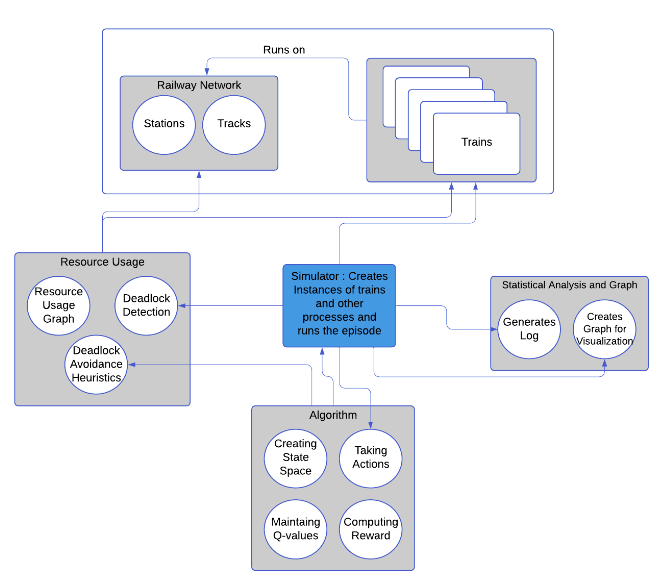
\includegraphics[width=1.0\textwidth]{Implementation}
    \caption{ Flow chart summarizing the implementation of railway simulator.  }
    \label{image-myimage1}
\end{figure}

\vspace{2cm}
\section{Modules and its components}
\begin{enumerate}
\item \textbf{Railway network and trains}

This is the main module that contains the basic architecture of railway network and the 
trains. Railway network consists of two basic components :-
\begin{itemize}
\item \textbf{Stations} : Stations in the railway network (synonymous to nodes in the network).
\item \textbf{Tracks} : Tracks connecting the stations (synonymous to edges in the network).
\end{itemize}
Once the railway network is created, train class (implemented as component) is used to create different instances
of the trains running over the network.

\item \textbf{Statistical Analysis and Graphs}

This module is responsible for creating the logs and generating necessary graphs for visualization 
and analysis.

\item \textbf{Resource Usage}

Whole railway network (station and tracks connecting the stations) is treated as pool of resource.
 Trains are ones that use this resource as they reside either on the station or the track. 
There are only fixed number of trains that can reside on the station and the track at a time.
It is also possible for the train to wait for a resource to free up, as it is occupied by other
trains. \textbf{Resource Usage Graph} component is responsible for generating the graph which show
what all resources are occupied by the trains and for what all resources train is waiting. This can be useful in detecting
deadlock.


There is another problem of deadlock which the simulator can run in. We are going to discuss this problem 
in full length in the later sections.\textbf{ Deadlock detection} and \textbf{deadlock avoidance} components
are used for detecting and avoiding the deadlock in the systems.

\item \textbf{Algorithm}

This module implements the algorithm (Q-Learning or Deep Q-learning) that helps in learning
the schedule. Currently only two components are implemented, creating state space and 
choosing action based on heuristic in \cite{ARTICLE:2}. More algorithms will be added in the future.

\item \textbf{Simulator}

This is one of the most important module that is responsible for creating all the processes 
that runs the simulator. It creates the environment and then invokes all the processes, then it handles 
further processing. Because of this module, we can add more modules in the future to the existing system.

\end{enumerate}







